\documentclass[11pt,a4paper]{article}

% packages
\usepackage[utf8]{inputenc}
\usepackage{amsmath}
\usepackage[T1]{fontenc}
\usepackage{setspace}
\usepackage{enumitem}
\usepackage{amsmath}
\usepackage{booktabs}
\usepackage{fullpage} 
\usepackage{tabularx}
\usepackage{amssymb, amstext, amsmath}
\usepackage{fancyhdr}
\usepackage{graphicx}
\usepackage{algorithmic}
\usepackage[ruled,vlined]{algorithm2e}
\usepackage{url}
\usepackage[bookmarks,unicode=true,pdftex,a4paper]{hyperref}
\usepackage[round]{natbib}
\usepackage[usenames,dvipsnames]{color, xcolor}
\headsep1cm

% macros
% misc
\newcommand\todo[1]{\textcolor{red}{TODO: #1}}
\newcommand\hide[1]{\textcolor{white}{#1}}

% formatting
\newcommand\bld[1]{\textbf{#1}}
\newcommand\ul[1]{\underline{#1}}
\newcommand\n[1]{\numprint{#1}}
\newcommand{\ts}{\textsuperscript}
\newcommand\red[1]{\textcolor{red}{#1}}
\newcommand\blue[1]{\textcolor{blue}{#1}}
\newcommand\link[2]{\href{#1}{\textcolor{blue}{\underline{#2}}}}

% sets
\newcommand\set[1]{\mathcal{#1}}
\newcommand\bb[1]{\mathbb{#1}}
\renewcommand\:{\colon} % for use with \sset, etc.
\newcommand{\sset}[1]{\left\{\,#1\,\right\}} % { ? }, automatic brackets
\newcommand{\ssets}[1]{\left\{#1\right\}} % {?}, automatic brackets
\newcommand{\ssetn}[1]{\{\,#1\,\}} % { ? }, normal brackets

% table formatting
% To better align bold entries in S columns (still broken)
% \usepackage{siunitx}
% \robustify\bfseries
% \newrobustcmd{\bfcell}{\bfseries}

% vector variables (taken from macros by Rainer Gemulla)
\newcommand\vect[1]{{\boldsymbol{#1}}}
\newcommand\va{\vect{a}}
\newcommand\vb{\vect{b}}
\newcommand\vc{\vect{c}}
\newcommand\vd{\vect{d}}
\newcommand\ve{\vect{e}}
\newcommand\vf{\vect{f}}
\newcommand\vg{\vect{g}}
\newcommand\vh{\vect{h}}
\newcommand\vi{\vect{i}}
\newcommand\vj{\vect{j}}
\newcommand\vk{\vect{k}}
\newcommand\vl{\vect{l}}
\newcommand\vm{\vect{m}}
\newcommand\vn{\vect{n}}
\newcommand\vo{\vect{o}}
\newcommand\vp{\vect{p}}
\newcommand\vq{\vect{q}}
\newcommand\vr{\vect{r}}
\newcommand\vs{\vect{s}}
\newcommand\vt{\vect{t}}
\newcommand\vu{\vect{u}}
\newcommand\vv{\vect{v}}
\newcommand\vw{\vect{w}}
\newcommand\vx{\vect{x}}
\newcommand\vy{\vect{y}}
\newcommand\vz{\vect{z}}
\newcommand\vzero{\vect{0}}
\newcommand\vone{\vect{1}}

\newcommand\valpha{\vect{\alpha}}
\newcommand\vbeta{\vect{\beta}}
\newcommand\veps{\vect{\epsilon}}
\newcommand\vdelta{\vect{\delta}}
\newcommand\vtheta{\vect{\theta}}
\newcommand\vsigma{\vect{\sigma}}
\newcommand\vpi{\vect{\pi}}
\newcommand\vlambda{\vect{\lambda}}

% matrix variables (taken from macros by Rainer Gemulla)
\newcommand\mA{\vect{A}}
\newcommand\mB{\vect{B}}
\newcommand\mC{\vect{C}}
\newcommand\mD{\vect{D}}
\newcommand\mE{\vect{E}}
\newcommand\mF{\vect{F}}
\newcommand\mG{\vect{G}}
\newcommand\mH{\vect{H}}
\newcommand\mI{\vect{I}}
\newcommand\mJ{\vect{J}}
\newcommand\mK{\vect{K}}
\newcommand\mL{\vect{L}}
\newcommand\mM{\vect{M}}
\newcommand\mN{\vect{N}}
\newcommand\mO{\vect{O}}
\newcommand\mP{\vect{P}}
\newcommand\mQ{\vect{Q}}
\newcommand\mR{\vect{R}}
\newcommand\mS{\vect{S}}
\newcommand\mT{\vect{T}}
\newcommand\mU{\vect{U}}
\newcommand\mV{\vect{V}}
\newcommand\mW{\vect{W}}
\newcommand\mX{\vect{X}}
\newcommand\mY{\vect{Y}}
\newcommand\mZ{\vect{Z}}
\newcommand\mzero{\vect{0}}

\newcommand{\mPi}{{\ensuremath{\vect{\Pi}}}}
\newcommand{\mSigma}{{\ensuremath{\vect{\Sigma}}}}
\newcommand{\mLambda}{{\ensuremath{\vect{\Lambda}}}}

% argmin, argmax
\DeclareMathOperator*{\argmin}{argmin} % amsmath package required
\DeclareMathOperator*{\argmax}{argmax} % amsmath package required

% matrix operations
\newcommand\xdiag{\operatorname{diag}}      
\newcommand\diag[1]{\xdiag\left(#1\right)}    % diagonal matrix


% header and footer
\lhead{Advanced Methods in Text Analytics, FSS 2025}
\chead{}
\rhead{\thepage\ }
\cfoot{}
\pagestyle{fancy}

\title{Advanced Methods in Text Analytics \\ 
Exercise 5: Transformers - Part 1\\
\textbf{Solutions}}
\author{Daniel Ruffinelli}
\date{FSS 2025}

\begin{document}
\maketitle

\section{Transformer Basics}

\begin{enumerate}[label=(\alph*)]
    \item Using dot-product attention over hidden representations $\vh_i$ with
          query $\vk$, we have:
          \begin{align*}
              \vc_k = \sum_j \alpha_j\vh_j,
          \end{align*}
          where $\alpha_j$ is defined as follows:
          \begin{align*}
              \alpha_j = \operatorname{softmax}(\vs)_j,
          \end{align*}
          and $s_j$ is given by:
          \begin{align*}
              s_j = \vk^T\vh_j.
          \end{align*}
          Components $s_j$ and $\alpha_j$ are the \emph{attention score} and
          \emph{attention weight} for input $j$, respectively.
          Due to the dot product used to compute attention scores, we have that
          $D = K$ and $\vc_k\in\bb{R}^D$, which is our context vector over $\mH$
          given query $\vk$.
          Note that from the transformers perspective, hidden representations
          $\vh_i$ are used as both (i) keys when computing $s_j$ and (ii) as
          values when computing $\vc_k$.
    \item The cost is $O(n^2)$ where $n$ is number of tokens in the input
          sequence for the case where attend to all tokens, or the number of
          previously seen tokens in the case where we attend only to tokens to
          the left.
          The cost is explained by the fact that each token attends to every
          other token in the sequence (or only those to the left).
          This is highly parallelizable, since computing the contextualized
          representation of each input token is indepedent of that same
          computation for every other token.
          This is easy to see when representing self-attention as matrix
          products, an operation that is highly parallelizable.

          Efforts exist to reduce this cost, e.g.\ using
          \href{https://arxiv.org/pdf/1904.10509v1.pdf}{\underline{sparse attention}}
          this cost is reduced to $O(n\sqrt{n})$.
          Other effors exist, such as the
          \href{https://arxiv.org/pdf/2009.14794.pdf}{\underline{performer models}},
          which use sparse factorizations of the self-attention projection
          matrices, or \href{https://arxiv.org/pdf/2105.03824.pdf}{\underline{FNet}},
          which replaces self-attention altogether with linear transformations
          based on Fourier transforms.
    \item
          \begin{enumerate}[label=(\roman*)]
              \item Here's an image depicting how sine and cosine functions
                    typically look like (source
                    \href{https://www.kapiert.de/sinus-und-kosinusfunktionen-eigenschaften/}{\textcolor{blue}{\underline{here}}}).
                    \begin{center}
                        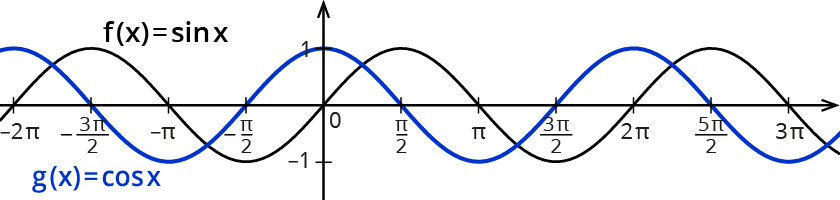
\includegraphics[scale=0.7]{img/sin_cos_2.png}
                    \end{center}
                    They are examples of periodic functions, i.e.\ functions
                    whose output values repeat in cycles.
                    Such functions are often described in terms of properties
                    such as frequency, period, etc.
                    We will define these properties as needed in the following.

                    The construction of positional embeddings only depends on
                    hyperparameters $n$ and $d$, so the resulting embedding for
                    position $k$ is the same no matter the input sequence.
                    This is something we want, as these embeddings should
                    encode positional information independently of factors such
                    as input sequence length.
                    The $i$-th row of the following matrix thus contains the
                    $i$-th positional embedding:
                    \begin{center}
                        $\begin{matrix}
                                0.000  & 1.000  & 0.000 & 1.000 \\
                                0.841  & 0.540  & 0.032 & 1.000 \\
                                0.909  & -0.416 & 0.063 & 0.998 \\
                                0.141  & -0.990 & 0.095 & 0.996 \\
                                -0.757 & -0.654 & 0.126 & 0.992
                            \end{matrix}$
                    \end{center}
                    The vectors are not large, as each element in this matrix is
                    close to zero.
                    This is so because the output of $\sin$/$\cos$ functions is
                    in the range $[-1,1]$.
                    Given that in the original architecture we \emph{add} these
                    positional embeddings to the token embeddings, we don't want
                    them to be large.
                    The translation that we apply to token embeddings via this
                    sum should be large enough to distinguish the same token
                    embeddings (which should encode semantics) when used in
                    different positions, but not too large that the position
                    information becomes a stronger signal to the model than the
                    semantics in the input sequence.
                    In addition, large positional vectors could introduce issues
                    during training, such as large gradients that are mostly
                    influenced by the position information, or similar issues
                    that the model may deal with by making token embeddings
                    small enough that they are too constrained to encode
                    semantic information well.
                    Note that such considerations may change if we use a
                    different operation to combine token embeddings with
                    position embeddings, e.g.\ concatenation.
              \item Since the frequency depends on $n,d,i$, each column of our PE
                    matrix is a sin/cos function with a fixed frequency.
                    If we look at each column as we increase values of $k$,
                    i.e.\ across rows, we see that elements change values as
                    we traverse the $\sin$/$\cos$ (the values of the lasts
                    columns also change, but this is less clear due to
                    rounding).
                    \begin{center}
                        $\begin{matrix}
                                0.000  & 1.000  & 0.000 & 1.000 & 0.000 & 1.000 & 0.000 & 1.000 & 0.000 & 1.000 \\
                                0.841  & 0.5409 & 0.158 & 0.987 & 0.025 & 1.000 & 0.004 & 1.000 & 0.001 & 1.000 \\
                                0.909  & -0.416 & 0.312 & 0.95  & 0.05  & 0.999 & 0.008 & 1.000 & 0.001 & 1.000 \\
                                0.141  & -0.990 & 0.458 & 0.889 & 0.075 & 0.997 & 0.012 & 1.000 & 0.002 & 1.000 \\
                                -0.757 & -0.654 & 0.592 & 0.806 & 0.100 & 0.995 & 0.016 & 1.000 & 0.003 & 1.000 \\
                                -0.959 & 0.284  & 0.712 & 0.702 & 0.125 & 0.992 & 0.020 & 1.000 & 0.003 & 1.000 \\
                                -0.279 & 0.960  & 0.814 & 0.581 & 0.150 & 0.989 & 0.024 & 1.000 & 0.004 & 1.000 \\
                                0.657  & 0.754  & 0.895 & 0.445 & 0.175 & 0.985 & 0.028 & 1.000 & 0.004 & 1.000 \\
                                0.989  & -0.146 & 0.954 & 0.298 & 0.200 & 0.980 & 0.032 & 0.999 & 0.005 & 1.000 \\
                                0.412  & -0.911 & 0.99  & 0.144 & 0.224 & 0.975 & 0.036 & 0.999 & 0.006 & 1.000
                            \end{matrix}$
                    \end{center}
                    In other words, the values in each column vary according to
                    a $\sin$/$\cos$ function.
                    For uneven values of $i$, we see that values start at $1$
                    and decrease as $k$ increases (cosine).
                    For even values of $k$, we see values increase from $0$
                    (sine).
                    This allows us to create vectors with different values for
                    contiguous features, i.e.\ vectors that are distinct from
                    one another, which is a good thing, because we want
                    \emph{each} of them to encode a \emph{different} position,
                    and these vectors are not learned.
                    We discuss the relation between $i$ and $k$, i.e.\ rows and
                    columns in the PE matrix, further in the next question.
              \item An example of how a sine function changes with increasing
                    frequencies is shown below (source
                    \href{https://antapex.org/mathnote4new.htm}{\textcolor{blue}{\underline{here}}}).
                    \begin{center}
                        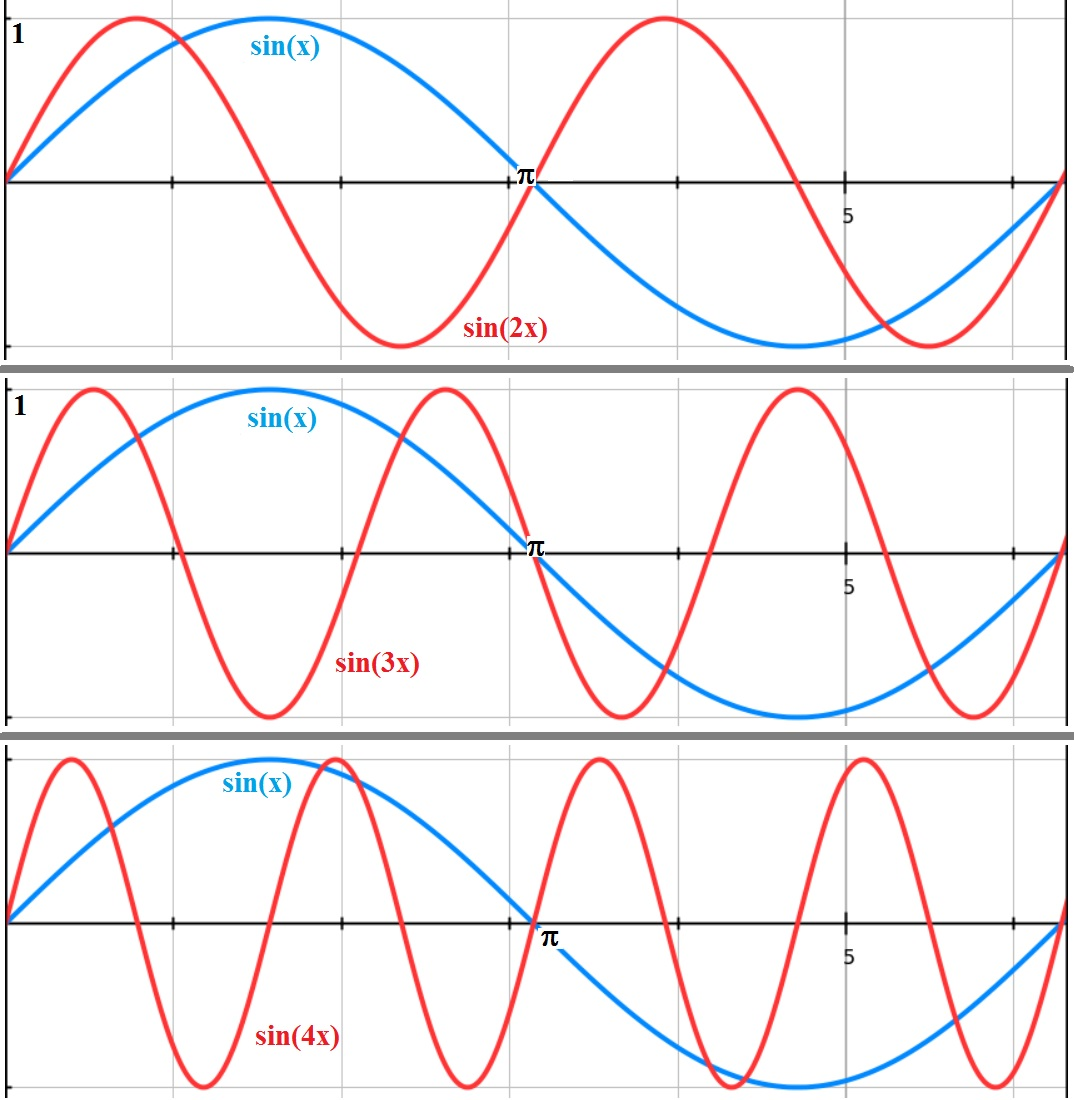
\includegraphics[scale=0.4]{img/sinuscosinus_10.jpg}
                    \end{center}
                    The columns, i.e.\ features, in our PE matrix change
                    following such patterns.
                    The higher the values of $i$, the lower the frequency and
                    the higher the period of these functions.
                    For example, for the values above, we have for
                    $i = [0, 1, 2, 3]$ the corresponding periods
                    $[6.28, 198.70, 6283.185, 198691.76]$.
                    With higher periods, the values that the same feature (column) in
                    our PE matrix takes across different rows (i.e.\ values of $k$)
                    change more slowly.
                    Thus, the rate of change for a given feature decreases with
                    increasing values of $i$ and we get more distinct features
                    across different values of $k$ (input positions) and across
                    different values of $i$ (positional embedding features).
                    This allows this non-parametric approach to use vectors
                    that are distinct from one another and each encode a
                    different position from 1 to some maximum input length.

                    Overall, this non-parametric approach for obtaining
                    positional embeddings is still useful for learning absolute
                    position embeddings (APE), but other variants exist.
                    BERT and GPT-3 use learned embeddings that encode APEs.
                    The T5 model learns relative positional embeddings with an
                    approach known as \emph{relative bias}, and more recent
                    models like PaLM and LLaMa use an approach called
                    \emph{rotary}, where they apply rotations to the query and
                    key embeddings that are proportional to the absolute
                    positions they want to encode.
                    There are
                    \href{https://arxiv.org/pdf/2305.19466.pdf}{\textcolor{blue}{\underline{studies}}}
                    that look into the differences of such approaches, and some
                    \href{https://aclanthology.org/2022.findings-emnlp.99.pdf}{\textcolor{blue}{\underline{works}}}
                    have suggested that causal language models do not require
                    positional embeddings, but still learn positional
                    information, which makes sense given the causal approach
                    to training and predicting that these models rely on.
          \end{enumerate}
\end{enumerate}

\section{Thinking about Perplexity}

\begin{enumerate}[label=(\alph*)]
    \item We have $p(X = i) = \frac{1}{6}$ so that:
          \begin{align*}
              H(x) = -\sum_{x=1}^6 \frac{1}{6}\log_2\left(\frac{1}{6}\right) \approx 2.58
          \end{align*}
          Entropy is a concept from information theory.
          We use this definition to define a bit: the entropy of a \emph{binary}
          random variable that takes values 0 or 1 with equal probability.
          We say we have gained 1 bit of information when the value of such a
          variable becomes known.
          When we define entropy using the natural logarithm (we can define it
          using any logarithm), we call such a unit of information a \emph{nat}.

          A more general intuition about entropy, and one commonly used in NLP,
          is what it tells us about the distribution represented by some random
          variable.
          Specifically, the higher the entropy, the more uniform the
          distribution.
          This is because the probability mass is distributed more evenly across
          the entire distribution, similar to how the physical entropy of a gas
          always increases to fill up the space it is contained in.
    \item We have:
          \begin{align*}
              ppl(x) = 2^{\left(-\sum_{x=1}^6 \frac{1}{6}\log_2\left(\frac{1}{6}\right)\right)} = 6
          \end{align*}
          This is the number of possible values our random variable can take.
          This is why, in the context of evaluating language models, perplexity
          can be interpreted as the number of possible next words given a word,
          often referred to as \emph{branching factor} (see Jurafsky Section
          3.2.1).

          In general, we can use any base for the logarithm when computing
          entropy, but we need to use that same base to compute perplexity.
          In code, we usually use $\ln$, which is why we use the exponential
          function to compute perplexity.
    \item We have:
          \begin{align*}
              H(w_1,w_2,\ldots,w_n) = -\sum_{w_{1:n}\in L} p(w_{1:n})\log p(X(w_{1:n}))
          \end{align*}
          The average entropy per word in the sequence, also known as
          \emph{entropy rate}, is given by:
          \begin{align*}
              H(w_1,w_2,\ldots,w_n) = -\frac{1}{n}\sum_{w_{1:n}\in L} p(w_{1:n})\log p(X(w_{1:n}))
          \end{align*}
          Note that we overload $H(x)$ to also represent entropy rate.
    \item The cross-entropy of some model $p$ of $m$ is defined as:
          \begin{align*}
              H(w_1,w_2,\ldots,w_n) = -\frac{1}{n}\sum_{w_{1:n}\in L} m(w_{1:n})\log p(w_{1:n}),
          \end{align*}
          where we set $w_{1:n} = X(w_{1:n})$ for simplicity.
          The intuition here is that we draw sequences from $m$, but we weigh
          them by their probability according to model $p$.
          In other words, this expectation (average information, i.e.\ entropy)
          is according to $p$.
          From a training perspective, $m$ is typically the target distribution
          that we want to learn with model $p$.
          In the case of entropy of sequences of text, you can think of $p$
          as the softmax distribution of a language model you are training,
          and $m$ the target distribution set by self-supervision (all the
          mass on a single word in the vocabulary).
    \item We proceed as follows:
          \begin{align*}
              ppl(W) & = 2^{H(W)}                                                                   \\
                     & = 2^{\left(-\frac{1}{N} \log p(W)\right)} &  & (\text{apply log properties}) \\
                     & = p(W)^{-\frac{1}{N}}.
          \end{align*}
          The approximation given in this question shows us not only how
          perplexity is related to entropy, but it also explains what we are
          doing when we compute the perplexity of a held-out validation corpus:
          We are estimating the cross-entropy of the entire language, where $p$
          is our language model and $m$ the true distribution of the language.
          Recall from machine learning courses, that cross-entropy is equivalent
          to log-loss, which explains why we typically apply the exponential
          function to our loss value to get perplexity in code ($\exp$ because
          we use $\ln$).
\end{enumerate}

To summarize, the takeaways from this task about perplexity are:
\begin{enumerate}
    \item Since we typically train language models with the cross-entropy loss,
          a.k.a.\ log loss, and we use $\ln$ to compute logarithms in code,
          applying the $\exp$ function to our loss gives us perplexity, because
          $ppl = e^{H(W)}$ according to Eq. 1 in the task description.
    \item The definition of perplexity from the lecture, i.e.\
          $p(W)^{\frac{1}{N}}$, is related to the definition of perplexity from
          information theory, i.e.\ $2^{H(W)}$ assuming log base 2, via the way
          to approximate the entropy of a language described in Eq. 2 in the 
          task description.
    \item The point above suggests that when computing the perplexity of a
          language model on a held-out corpus, we are estimating the 
          cross-entropy of the entire language used in the validation corpus.
          Since the larger the $N$ in Eq. 2, the better the estimate, we want 
          to use a large enough validation corpus.
\end{enumerate}

\end{document}
